\documentclass[11pt]{article}
\usepackage[margin=2.2cm]{geometry}
\usepackage{graphicx,booktabs,caption,float,amsmath}
\captionsetup{font=small}
\title{CS6600 Assignment 2: Branch Predictor Simulator}
\author{Shubham Jadhav (CS24S009)}
\date{}
\begin{document}
\maketitle

\section{Simulator and validation}
\texttt{branch\_predictor.cpp} implements a bimodal predictor (a table of $2^m$ 2-bit saturating counters indexed by PC bits $m{+}1..2$) and a gshare predictor (the upper $n$ of the $m$ index bits are XORed with an $n$-bit global history register; the history shifts in the actual outcome from the most significant end). All counters start at 2 (weakly taken). All 6 validation runs and the 2 sample runs match the reference outputs under a plain \texttt{diff -iw}, and 40 random bimodal and gshare configurations ($2\le m\le 16$, $0\le n\le m$, both traces) match an independent model of the same specification, including the final table contents. Gshare with $n=0$ reproduces the bimodal predictor exactly.

A table of $2^m$ counters costs $2^{m+1}$ bits $=2^{m-2}$ bytes, so the 16~kB budget allows $m\le 16$. The required plots cover $7\le m\le 12$; to choose designs within the budget the sweep is also run up to $m=16$ (dashed or in the extended plots). Both traces have 2{,}000{,}000 branches.

\section{Bimodal predictor}
\begin{figure}[H]\centering
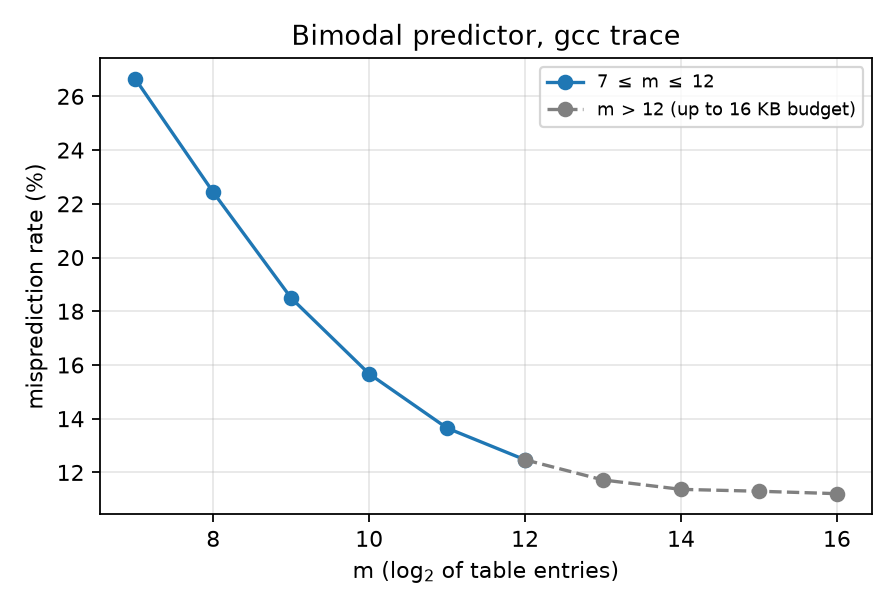
\includegraphics[width=.49\linewidth]{SimulationGraphs/Bimodal_gcc_benchmark.png}\hfill
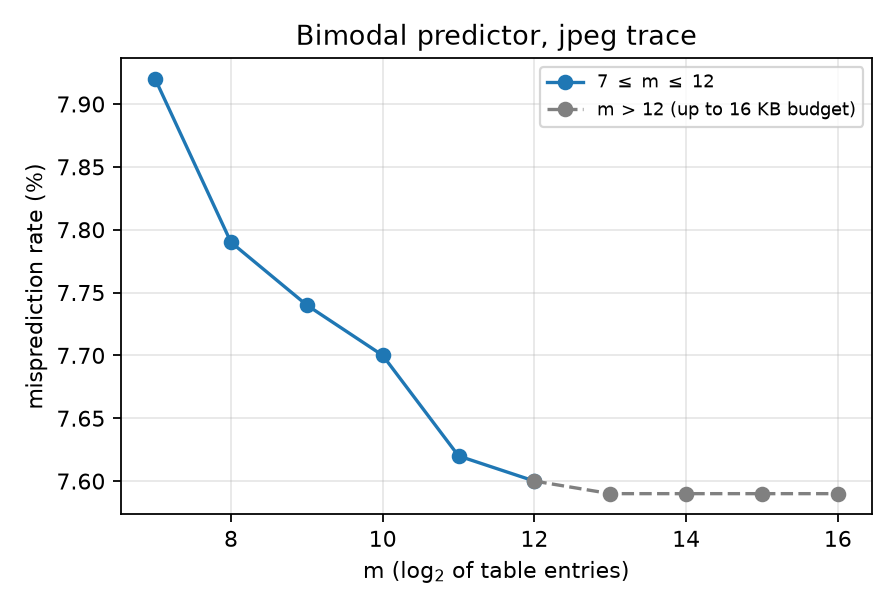
\includegraphics[width=.49\linewidth]{SimulationGraphs/Bimodal_jpeg_benchmark.png}
\caption{Misprediction rate versus $m$ for the bimodal predictor (solid: required range, dashed: up to the 16~kB budget).}
\end{figure}
\paragraph{Trends.} For \textbf{gcc} the rate falls steeply and monotonically: 26.65\% at $m=7$, 15.67\% at $m=10$, 12.47\% at $m=12$ and 11.21\% at $m=16$. Each doubling of the table helps less (gains of 4.2, 3.9, 2.8, 2.0, 1.2, 0.75, 0.35, 0.07 and 0.09 points for $m=7\to8,\dots,15\to16$), which shows that gcc has thousands of active static branches and a small table mostly causes \emph{aliasing}. For \textbf{jpeg} the curve is nearly flat: 7.92\% at $m=7$ to 7.60\% at $m=12$ and 7.59\% from $m=13$ on. jpeg runs a small set of loop branches that fit in a tiny table; its remaining mispredictions are data-dependent branches that no table size removes. The two benchmarks differ in both level (jpeg is already at 7.9\% with 128 entries, while gcc needs 4096 entries to reach 12.5\%) and in sensitivity (gcc improves by 14.2 points over $7\le m\le12$, jpeg by 0.3).

\paragraph{Proposed designs (16~kB budget).} The knee is where a doubling buys less than about 0.4 points.
\begin{center}\small\begin{tabular}{lcccc}\toprule
Benchmark & Proposed $m$ & Storage & Misprediction rate & Best within budget ($m=16$)\\\midrule
gcc & 14 & 4~kB & 11.37\% & 11.21\% (16~kB)\\
jpeg & 11 & 512~B & 7.62\% & 7.59\% ($m\ge13$)\\\bottomrule
\end{tabular}\end{center}
For gcc, $m=14$ is within 0.16 points of the 16~kB table for a quarter of the storage; $m=12$ (1~kB, 12.47\%) is the cheaper choice if 1.1 points can be given up. For jpeg, $m=11$ is within 0.03 points of the floor; going to $m=13$ would only double the table for no further gain.

\section{Gshare predictor}
\begin{figure}[H]\centering
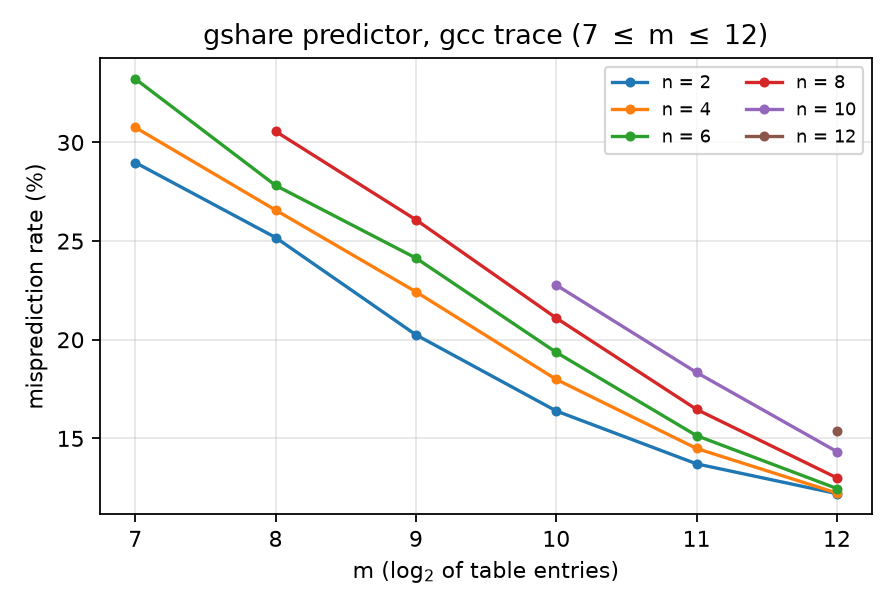
\includegraphics[width=.49\linewidth]{SimulationGraphs/Gshare_gcc_benchmark.png}\hfill
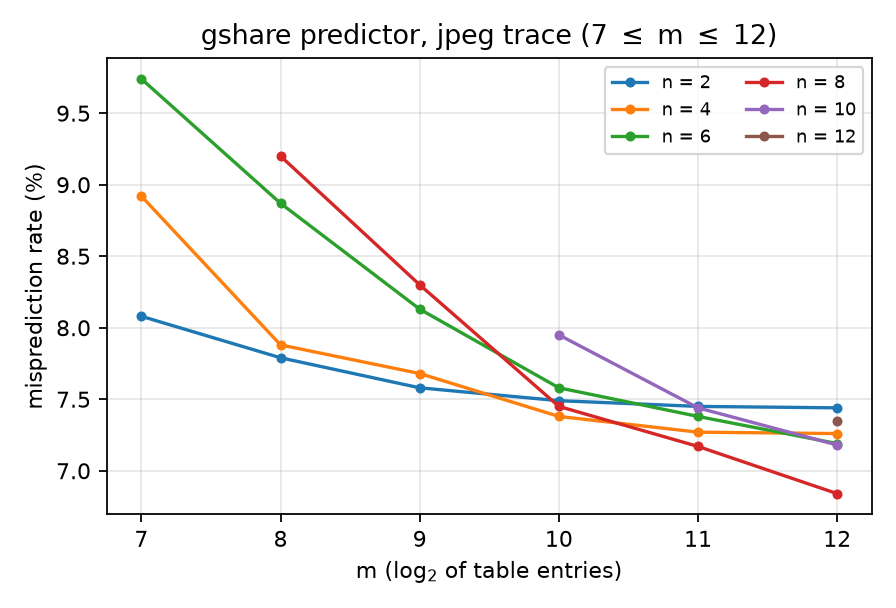
\includegraphics[width=.49\linewidth]{SimulationGraphs/Gshare_jpeg_benchmark.png}
\caption{Gshare misprediction rate versus $m$, one curve per even $n$ (only legal $m\ge n$), $7\le m\le 12$.}
\end{figure}
\begin{figure}[H]\centering
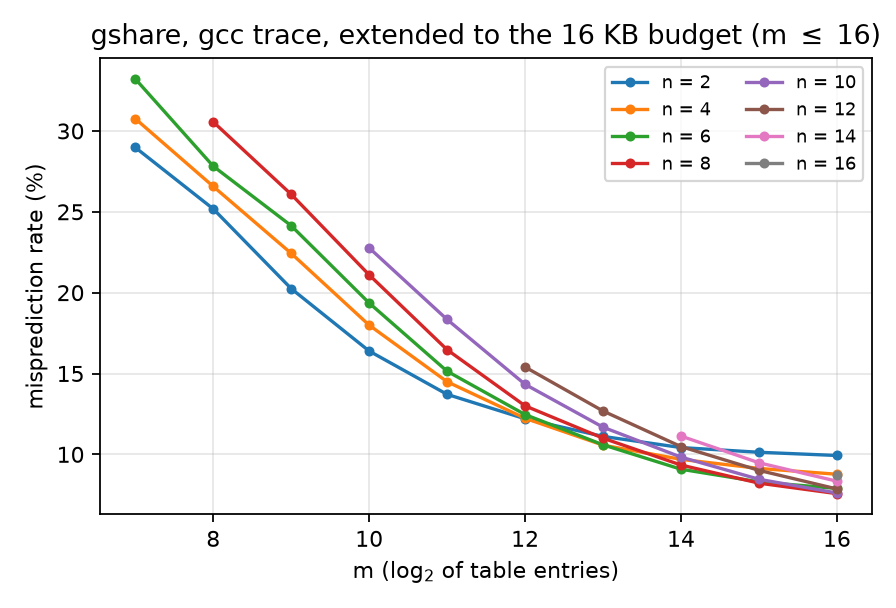
\includegraphics[width=.49\linewidth]{SimulationGraphs/Gshare_gcc_extended.png}\hfill
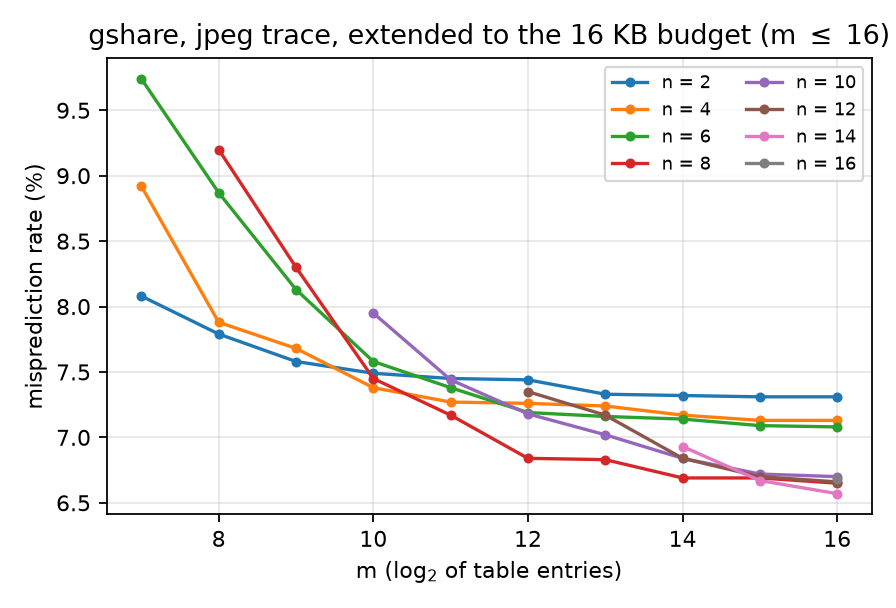
\includegraphics[width=.49\linewidth]{SimulationGraphs/Gshare_jpeg_extended.png}
\caption{The same sweep extended to the 16~kB budget ($m\le 16$, even $n\le 16$).}
\end{figure}

\paragraph{Trends, gcc.} At a fixed $m$ the best $n$ depends on the table size. In small tables extra history only hurts: at $m=8$ the rate is 25.2\% for $n=2$ but 30.6\% for $n=8$; at $m=12$ it grows from 12.20\% ($n=2$) to 15.40\% ($n=12$). History bits are XORed into the upper index bits, so each static branch spreads over $2^n$ entries; in a small table that multiplies aliasing and training time faster than correlation helps. In large tables the sign flips: at $m=16$ the order reverses and $n=8$ (7.57\%) and $n=10$ (7.61\%) beat $n=2$ (9.93\%). Every curve keeps falling with $m$ (the larger-$n$ curves fastest), so unlike bimodal there is no knee inside the 16~kB budget. \textbf{Comparison with bimodal:} bimodal is better up to $m=10$ (e.g.\ 15.67\% against at best 16.39\% at $m=10$), the two are equal at $m=11$ (13.65\% vs.\ 13.71\%), and from $m=12$ gshare wins by more and more (7.57\% vs.\ 11.21\% at $m=16$, 32\% fewer mispredictions).

\paragraph{Trends, jpeg.} The differences are an order of magnitude smaller. Small-$n$ curves are flat (7.3--8.1\%); large $n$ is worse in tiny tables (9.74\% for $n=6$ at $m=7$) but becomes the best once the table is big enough: $n=8$ reaches 6.84\% at $m=12$ and 6.65\% at $m=16$, and the overall best is 6.57\% at $(m,n)=(16,14)$. jpeg's loops have long, regular patterns, so a long history identifies the iteration, while gcc's branch behaviour is dominated by capacity and aliasing. Gshare beats the bimodal floor of 7.59\% by up to 13\%, but, unlike for gcc, the gain is small in absolute terms (1 point).

\paragraph{Proposed designs (16~kB budget).}
\begin{center}\small\begin{tabular}{lcccc}\toprule
Benchmark & $(m,n)$ & Storage & Misprediction rate & Reference points\\\midrule
gcc & (16, 8) & 16~kB & 7.57\% & best even $n$ at $m=16$; overall best (16, 9) 7.49\%\\
 & (14, 8) & 4~kB & 9.34\% & cheaper alternative (4$\times$ less storage than the best bimodal and 17\% fewer mispredictions)\\
jpeg & (14, 8) & 4~kB & 6.69\% & within 0.12 of the best, (16, 14) 6.57\%\\
 & (12, 8) & 1~kB & 6.84\% & within 0.27 of the best, 4$\times$ less storage\\\bottomrule
\end{tabular}\end{center}
For gcc I would use $(16,8)$: the budget is the only constraint and the curve is still falling at $m=16$, while $(15,8)$ at 8~kB loses 0.65 points (8.22\%). For jpeg the curve is flat after $m=12$: the 4~kB design $(14,8)$ is within 0.12 points of the best and uses a quarter of the budget.

\end{document}
